%%
%% This is file `sample-acmlarge.tex',
%% generated with the docstrip utility.
%%
%% The original source files were:
%%
%% samples.dtx  (with options: `acmlarge')
%% 
%% IMPORTANT NOTICE:
%% 
%% For the copyright see the source file.
%% 
%% Any modified versions of this file must be renamed
%% with new filenames distinct from sample-acmlarge.tex.
%% 
%% For distribution of the original source see the terms
%% for copying and modification in the file samples.dtx.
%% 
%% This generated file may be distributed as long as the
%% original source files, as listed above, are part of the
%% same distribution. (The sources need not necessarily be
%% in the same archive or directory.)
%%
%% The first command in your LaTeX source must be the \documentclass command.
\documentclass[sigconf]{acmart}

%%
%% \BibTeX command to typeset BibTeX logo in the docs
\AtBeginDocument{%
  \providecommand\BibTeX{{%
    \normalfont B\kern-0.5em{\scshape i\kern-0.25em b}\kern-0.8em\TeX}}}

%% Rights management information.  This information is sent to you
%% when you complete the rights form.  These commands have SAMPLE
%% values in them; it is your responsibility as an author to replace
%% the commands and values with those provided to you when you
%% complete the rights form.
%% TODO review later

% \setcopyright{acmcopyright}
% \copyrightyear{2018}
% \acmYear{2018}
% \acmDOI{10.1145/1122445.1122456}


%%
%% These commands are for a JOURNAL article.
%% TODO review later
% \acmJournal{POMACS}
% \acmVolume{37}
% \acmNumber{4}
% \acmArticle{111}
% \acmMonth{8}

%%
%% Submission ID.
%% Use this when submitting an article to a sponsored event. You'll
%% receive a unique submission ID from the organizers
%% of the event, and this ID should be used as the parameter to this command.
%%\acmSubmissionID{123-A56-BU3}

%%
%% The majority of ACM publications use numbered citations and
%% references.  The command \citestyle{authoryear} switches to the
%% "author year" style.
%%
%% If you are preparing content for an event
%% sponsored by ACM SIGGRAPH, you must use the "author year" style of
%% citations and references.
%% Uncommenting
%% the next command will enable that style.
%%\citestyle{acmauthoryear}
\graphicspath{ {./images/} }
\DeclareGraphicsExtensions{.png}
% \usepackage{cite}
% \usepackage[pdftex]{hyperref}
% \usepackage{xcolor}
% \hypersetup{
%     colorlinks,
%     linkcolor={red!50!black},
%     citecolor={blue!50!black},
%     urlcolor={blue!80!black}
% }
\usepackage[autostyle]{csquotes}

%encoding
%--------------------------------------
\usepackage[T1]{fontenc}
\usepackage[utf8]{inputenc}
%--------------------------------------

%Portuguese-specific commands
%--------------------------------------
\usepackage[portuguese]{babel}
%--------------------------------------

%Hyphenation rules
%--------------------------------------
\usepackage{hyphenat}
\hyphenation{mate-mática recu-perar}
%--------------------------------------
 


\usepackage{titlesec}

\setcounter{secnumdepth}{4}

\titleformat{\subsubsection}
{\normalfont\normalsize\bfseries}{\thesubsubsection}{1.2em}{}
\titlespacing*{\subsubsection}
{0pt}{3.25ex plus 1ex minus .2ex}{1.5ex plus .2ex}

\titleformat{\paragraph}
{\normalfont\normalsize\bfseries}{\theparagraph}{1em}{}
\titlespacing*{\paragraph}
{0pt}{3.25ex plus 1ex minus .2ex}{1.5ex plus .1ex}

%%
%% end of the preamble, start of the body of the document source.
\begin{document}


%%
%% The "title" command has an optional parameter,
%% allowing the author to define a "short title" to be used in page headers.
\title{Pesquisa sobre práticas de Integração e Implantação contínuas em Recife}

%%
%% The "author" command and its associated commands are used to define
%% the authors and their affiliations.
%% Of note is the shared affiliation of the first two authors, and the
%% "authornote" and "authornotemark" commands
%% used to denote shared contribution to the research.
% \author{Mateus Valgueiro Teixeira}
% \email{mvt@cin.ufpe.br}
% \orcid{1234-5678-9012}
% \affiliation{%
%   \institution{Centro de Informatica}
%   \streetaddress{Av. Jorn. Aníbal Fernandes}
%   \city{Recife}
%   \state{Pernambuco}
%   \country{Brazil}
% }

% \author{Heitor Sammuel Carvalho Souza}
% \email{hssc@cin.ufpe.br}
% \orcid{1234-5678-9012}
% \affiliation{%
%   \institution{Centro de Informatica}
%   \streetaddress{Av. Jorn. Aníbal Fernandes}
%   \city{Recife}
%   \state{Pernambuco}
%   \country{Brazil}
% }

% \author{Paulo Borba}
% \email{phmb@cin.ufpe.br}
% \orcid{1234-5678-9012}
% \affiliation{%
%   \institution{Centro de Informatica}
%   \streetaddress{Av. Jorn. Aníbal Fernandes}
%   \city{Recife}
%   \state{Pernambuco}
%   \country{Brazil}
% }

% \author{Klissiomara Lopes Dias}
% \email{kld2@cin.ufpe.br}
% \orcid{1234-5678-9012}
% \affiliation{%
%   \institution{Centro de Informatica}
%   \streetaddress{Av. Jorn. Aníbal Fernandes}
%   \city{Recife}
%   \state{Pernambuco}
%   \country{Brazil}
% }

%%
%% By default, the full list of authors will be used in the page
%% headers. Often, this list is too long, and will overlap
%% other information printed in the page headers. This command allows
%% the author to define a more concise list
%% of authors' names for this purpose.
% \renewcommand{\shortauthors}{Mateus Valgueiro et al.}

%%
%% The abstract is a short summary of the work to be presented in the
%% article.
\resumo

As práticas de \emph{Continuous Integration} [CI], \emph{Continuous Delivery} e \emph{Continuous Deployment} [CD] já estão presentes no cotidiano de grandes empresas de todo o mundo. E isto é devido, entre outras coisas, aos comprovados benefícios que a utilização destas técnicas trazem para a equipe e para o produto em desenvolvimento. Mesmo assim, poucos são os estudos que investigam o estado da arte destas práticas na maioria das empresas, principalmente no contexto da cidade de Recife.  Com isso, o presente trabalho objetiva entender como as técnicas de integração, entrega e implantação contínuas foram importadas para as empresas recifenses, assim como identificar princípios e práticas adjacentes que governam a adoção destas técnicas. Para tanto, foi realizada uma pesquisa qualitativa por meio de entrevistas com 11 desenvolvedores de software de empresas de tecnologia sediadas na cidade do Recife. Foi descoberto que a amostra não segue o \emph{Stairway to Heaven}, teoria definida pelo artigo base deste trabalho e que sugere que a adoção deve seguir uma sequência específica de práticas. Não obstante, a maioria entrevistada integra o código de uma nova funcionalidade para a \emph{branch} principal apenas no final da \emph{Sprint}, não diariamente, o que não é consistente com as definições mais comuns de CI. Além disso, a prática de Testes A/B não foi encontrada em nenhum dos times entrevistados, em razão da baixa quantidade de usuários ativa ou por não se aplicar ao contexto da aplicação.

% Palavras-chave do resumo em Português
\begin{keywords}
    Integração Contínua, Deployment Contínuo, Desenvolvimento Colaborativo, Engenharia de Software
\end{keywords}


%%
%% The code below is generated by the tool at http://dl.acm.org/ccs.cfm.
%% Please copy and paste the code instead of the example below.
%%
% \begin{CCSXML}
% <ccs2012>
%  <concept>
%   <concept_id>10010520.10010553.10010562</concept_id>
%   <concept_desc>Computer systems organization~Embedded systems</concept_desc>
%   <concept_significance>500</concept_significance>
%  </concept>
%  <concept>
%   <concept_id>10010520.10010575.10010755</concept_id>
%   <concept_desc>Computer systems organization~Redundancy</concept_desc>
%   <concept_significance>300</concept_significance>
%  </concept>
%  <concept>
%   <concept_id>10010520.10010553.10010554</concept_id>
%   <concept_desc>Computer systems organization~Robotics</concept_desc>
%   <concept_significance>100</concept_significance>
%  </concept>
%  <concept>
%   <concept_id>10003033.10003083.10003095</concept_id>
%   <concept_desc>Networks~Network reliability</concept_desc>
%   <concept_significance>100</concept_significance>
%  </concept>
% </ccs2012>
% \end{CCSXML}

% \ccsdesc[500]{Computer systems organization~Embedded systems}
% \ccsdesc[300]{Computer systems organization~Redundancy}
% \ccsdesc{Computer systems organization~Robotics}
% \ccsdesc[100]{Networks~Network reliability}

%%
%% Keywords. The author(s) should pick words that accurately describe
%% the work being presented. Separate the keywords with commas.


%%
%% This command processes the author and affiliation and title
%% information and builds the first part of the formatted document.
\maketitle


\section{Introdução}

As práticas de integração, entrega e implantação contínuos \cite{fowlerCI, fowlerCD} (\emph{Continuous Integration} [CI], \emph{Continuous Delivery} e \emph{Continuous Deployment} [CD]) já são muito difundidas e utilizadas por empresas de tecnologia em todo o mundo. Segundo a pesquisa da empresa \emph{digital.ia}\cite{stateAgileReport2020}, 55\% dos participantes reportaram que sua organização utiliza a técnica de integração contínua. Também nesta mesma pesquisa foi encontrado que 41\% utilizam a técnica de \emph{Continuous Delivery} e 36\%, \emph{Continuous Deployment}.

Estes números elevados são causados principalmente pelos benefícios que a utilização destas técnicas trazem para a equipe e para o produto em desenvolvimento. Estudos comprovam que os desenvolvedores envolvidos se sentem mais produtivos quando usam as práticas de CI/CD \cite{hilton2016} e o seu uso traz maior qualidade ao software que está sendo produzido \cite{savor2015}. 

É possível, no entanto, perceber uma grande falta de estudos a respeito de como essas práticas foram importadas para as empresas de todo o mundo \cite{empiricalStudy2016}, incluindo Recife -- as pesquisas são geralmente voltadas apenas para as corporações globais como Facebook \cite{savor2015} e Google \cite{googleCi}. A capital pernambucana é um dos grandes pólos tecnológicos do Brasil: somente no Porto Digital, localizado na cidade, há cerca de 330 empresas e 11 mil trabalhadores, com faturamento anual de R\$ 2,3 bilhões em 2019 \cite{portoDigital}.

Um estudo a respeito de como as técnicas de CI/CD migraram para a indústria de Recife serve como ponto de partida para pesquisas relacionadas ao levantamento de dores sentidas pelos desenvolvedores locais que inibem a utilização destas técnicas.

Neste contexto, este trabalho tem como objetivo entender, através de uma pesquisa qualitativa, quais as práticas e técnicas subjacentes de integração, entrega e \emph{deployment} contínuos adentraram nas empresas de Recife. Não obstante, o trabalho deseja descobrir que princípios e práticas subjacentes governam a adoção destas técnicas.



\chapter{Motivação}
Neste cápitulo será abordada a motivação por trás da pesquisa produzida. Na primeira seção, será falado um pouco sobre a grande adoção das práticas ágeis pela indústria. Já na segunda seção, será abordada a falta de estudos voltados para o contexto Recifense. A terceira discorre sobre o artigo base que serviu de motivação para este trabalho. A última seção contém as perguntas de pesquisa que este trabalho tenta responder.

\section{A grande adoção de CI e CD}
As práticas de integração e \emph{deployment} contínuos (\emph{Continuous Integration} e \emph{Continuous Deployment}) já são muito difundidas e utilizadas por empresas de tecnologia em todo o mundo. Segundo \cite{stateAgileReport2020}, 95\% dos participantes reportaram que sua organização pratica metodologias ágeis de desenvolvimento e 55\% utilizam a técnica de integração continua. Também nesta mesma pesquisa foi encontrado que 36\% utilizam a técnica de \emph{deployment} contínuos. 

Estes números elevados são causados principalmente pelos benefícios que a utilização destas técnicas trazem para a equipe e para o produto em desenvolvimento. Ainda de acordo com \cite{stateAgileReport2020}, entre as razões para adoção de CI/CD, as principais são aceleração de entregas de software (71\%), e aumentar a produtividade (51\%) e a qualidade do software (42\%). 

Especificamente sobre integração contínua, a prática hoje em dia já é bastante estudada difundida na indústria. O estudo \cite{hilton2016} comenta que desenvolvedores envolvidos se sentem mais produtivos quando utilizam a prática e dão mais valor aos testes automáticos.  Já com relação a \emph{deployment} contínuo, o estudo \cite{savor2015} mostra que seu uso traz maior qualidade ao software que está sendo produzido. 

\section{A falta de estudos no contexto Recifense}

Ainda há, no entanto, uma grande falta de estudos a respeito de como essas práticas se exportaram para as grandes empresas \cite{empiricalStudy2016}, inclusive em Recife, um dos grandes polos tecnológicos do Brasil. Somente no Porto Digital, localizado na capital pernambucana, há cerca de 330 empresas e 11 mil trabalhadores com faturamento anual de R\$ 2,3 bilhões somente em 2019 \cite{portoDigital}.

% TODO adicionar artigos sobre recife(?)

\section{O artigo base}
Com o objetivo de entender um pouco mais sobre o estado das práticas de CI/CD no contexto de Recife, nos baseamos no estudo \cite{empiricalStudy2016}, que busca entender como as práticas geralmente associadas a \emph{Continuous Deployment} acharam o seu caminho na indústria européia e norte-americana. Para tal, foi utilizado um método misto de estudo empírico baseado em um pré-estudo na literatura, entrevistas qualitativas com 20 participantes e uma entrevista quantitativa que recebeu 187 respostas. A ideia era questionar até que ponto a sabedoria na area estava dominada por peculiaridades de um pequeno grupo de grandes empresas, como Facebook e Google.

Durante o trabalho os autores definem a \emph{stairway to heaven} (escada para o céu, em tradução livre), que tem como objetivo definir um caminho de evolução das empresas para um estágio de entregas sofisticado. Esta permeia práticas de integração contínua, \emph{deployment} contínuo e entregas parciais e 

\begin{figure}[ht]
\begin{center}
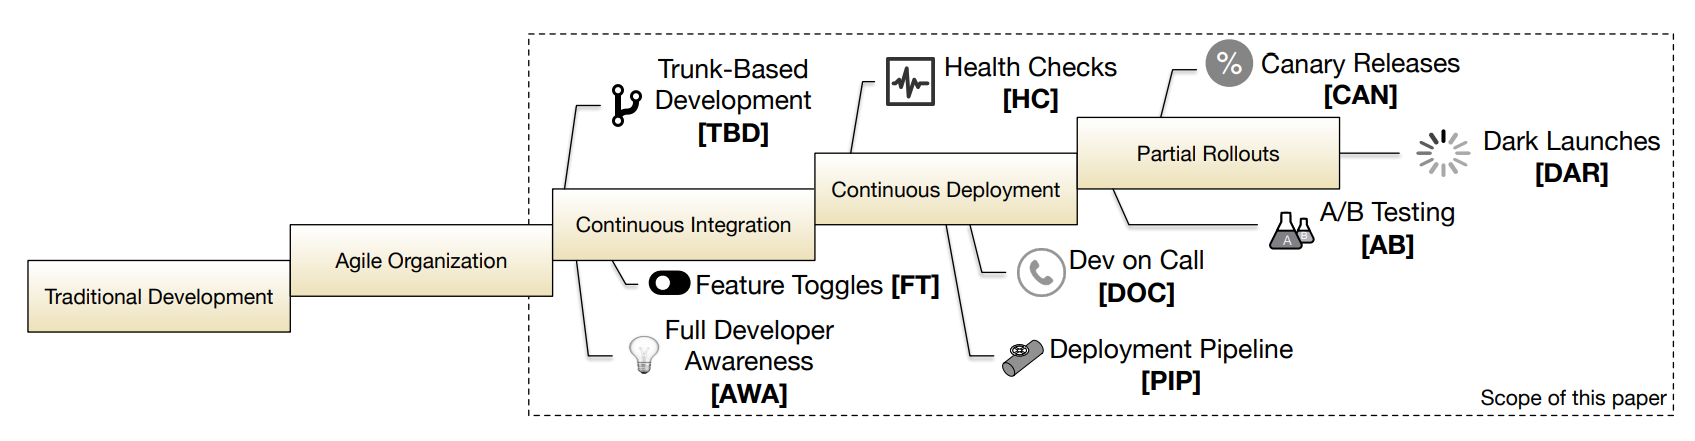
\includegraphics[width=\textwidth]{stairway_to_heaven.png}
\end{center}
\caption[Stairway to Heaven]{
    A escada de evolução denominada "Stairway to Heaven" proposta pelo artigo base.
    Fonte: Schermman et al (2016)
}\label{fig_exe}

\end{figure}

Com este caminho definido, os autores do artigo montaram as entrevistas qualitativas e quantitativas baseadas nas práticas que surgiram em cada degrau da evolução. O interessante da abordagem dos autores foi o roteiro consistir de perguntas sobre o processo utilizado, sem perguntar diretamente se o entrevistado utiliza determinada prática. Isso faz com que os resultados baseiem-se em um conjunto contido de definições, excluindo concepções diversas que pessoas diferentes possam ter a respeito de um mesmo assunto.

\section{Perguntas de pesquisa} 
Assim, a grande adoção da indústria mundial das práticas de CI/CD, aliado a pequena quantidade de trabalhos a respeito no contexto recifense e a excelente metodologia proposta pelo artigo de Schermman et al \cite{empiricalStudy2016} foram as principais motivações para o desenvolvimento deste trabalho. Para este as seguintes perguntas de pesquisa foram formadas:

\begin{enumerate}
\item Quais as práticas de CI/CD são utilizadas pelas empresas em Recife?
\item O cenário de CI/CD nas empresas em recife segue o \emph{stairway to heaven} proposto no artigo?
\item Quais são os princípios e práticas subjacentes que governam a adoção de CD na indústria?
\end{enumerate}

Para responder as perguntas acima foi decido reaplicar a pesquisa qualitativa do artigo \cite{empiricalStudy2016} com desenvolvedores recifenses, baseando-se também na mesma lista de definições de cada uma das práticas envolvidas no "stairway to heaven". A pesquisa qualitativa neste contexto foi considerada fundamental para garantir que os entrevistados entendessem claramente as perguntas e excluir possíveis entendimentos errados de termos em inglês, linguagem não nativa de todos os participantes. Vale salientar que não foi replicado a pesquisa quantitativa presente no artigo base, mas esta pode servir como um trabalho futuro a este.

Além disso, as perguntas 1 e 3 são bem parecidas com as perguntas de pesquisa do artigo base, mas incluindo a técnica de \emph{Continuous Integration}. Não obstante, uma terceira pergunta foi adicionada (\emph{RQ2}), que foca na escada de evolução proposta pelo artigo. Ela tenta responder se a \emph{stairway to heaven} é seguida no contexto de Recife, visto que, no outro, os próprios autores já refutaram esta definição com os seus resultados.



% \section{Definições}

Para este trabalho foram utilizados as mesmas definições levantadas pelo artigo base.

\subsection{Integração Contínua}
A técnica de integração contínua (CI), de acordo com \cite{fowlerCI}, têm como principal característica a integração de código no repositório compartilhado múltiplas vezes por dia. Para garantir a qualidade do software que está sendo integrado, cada \emph{merge} passa por testes automáticos pré-programados que garantem que cenários de usabilidade estão de acordo com os requisitos definidos. 

Algumas práticas foram definidas dentro da técnica para definir processos chaves que produzem um CI eficiente. Entre elas, temos o \emph{trunk based development} [TBD] \cite{devAndDeploymentFB}, onde todo o time contribui para uma única \emph{branch} no repositório de versionamento, chamada usualmente de \emph{main}. Esta técnica é comumente utilizada para diminuir a quantidade de conflitos entre linhas de códigos que estão sendo concorrentemente modificadas por desenvolvedores diferentes. 

Para garantir que o \emph{trunk based development} funcione como esperado, deve-se ter uma ferramenta que possibilite o chaveamento de partes de código que ainda não foram finalizadas. A implementação comum desta técnica é \emph{feature toggle} [FT] \cite{featureToggles}. A técnica define, através de condicionais adicionadas no código fonte, que blocos devem ser executados ou ignorados no ambiente de produção.

Outra prática relacionada a técnica de integração contínua é o chamado \emph{developer awareness} [AWA] \cite{awa}, que prega a quebra de silos entre os desenvolvedores e processos de \emph{release}, o status dos ambientes e informações gerais da infraestrutura do sistema que está sendo desenvolvido. A ideia é não depender de um time específico de fora para cuidar de questões arquiteturais e do processo de entrega, mas sim difundir o conhecimento entre todos os envolvidos no desenvolvimento. Este é um dos conceitos recomendados na cultura \emph{DevOps} comentada anteriormente.

\subsection{Entrega e Implantação Contínuas}

A técnica de \emph{entrega contínua} define que o software tem que estar a qualquer momento pronto para ser enviado para produção no repositório principal \cite{fowlerCD}. Para que a técnica de entrega contínua funcione como o esperado, é necessário principalmente que o software esteja pronto para \emph{implantação} durante todo o ciclo de vida e que o time sempre priorize deixar o código pronto para produção ao invés de priorizar novas funcionalidades.

Muitas vezes a técnica de \emph{entrega contínua} é confundida com a de \emph{implantação contínua}. No entanto, esta última significa que o código é automaticamente colocado em produção sempre que possível, resultando em múltiplas implantações por dia. Com a entrega contínua, a empresa pode escolher ter uma frequência de implantações mais lenta, mesmo tendo o software sempre pronto para utilização. Outro ponto importante é que para se ter implantação contínua, é necessário ter entrega contínua.

A técnica de implantação contínua foi bastante difundida através do exemplo de empresas como a \emph{Flickr}, que em 2009 comentou sobre suas mais de 10 implantações diárias \cite{flickrTalk}, antes mesmo do termo \emph{DevOps} ser inventado. 

Algumas práticas definem alguns dos passos necessários para utilizar a técnica de CD. Podemos citar a \emph{deployment pipeline} (pipeline de implantação) [PIP] \cite{devopsBook}, que define o conjunto de passos que qualquer mudança de código tem que passar para chegar em produção. Esses passos podem tratar da compilação do código, da execução de testes em diferentes ambientes, entre outras coisas e pode ser totalmente ou parcialmente automatizada. Idealmente, o conjunto de passos deve ser automatizado o máximo possível para garantir rapidez e confiabilidade dos processos envolvidos.

Depois da entrega de uma nova versão, \emph{health checks} [HC] \cite{devopsBook} são necessários para garantir que o produto está funcionando corretamente. O sistema tem uma série de parâmetros definidos pela equipe que mostram se há algum problema no ambiente de produção, por exemplo, falha na conexão com o banco de dados, serviços inativos, certificados HTTPS expirados, entre outros. Muitas vezes o sistema tem a funcionalidade de envio de mensagens para os responsáveis quando algo de errado ocorre no ambiente.

Para garantir ainda mais uma colaboração maior entre desenvolvedores e o time de operações, surgiu a prática de \emph{developer on call} [DOC] \cite{devAndDeploymentFB}. Esta sugere que o desenvolvedor responsável pela funcionalidade recém lançada fique disponível por tempo extra após o lançamento em produção. Caso haja algum erro, ele será a pessoa mais propícia a resolvê-lo o mais rápido possível.

\subsection{Entregas Parciais}

A prática de \emph{partial rollouts} (ou entregas parciais) pode ser definida como um processo de garantia de qualidade e validação de requisitos que ocorrem em tempo de execução \cite{empiricalStudy2016}. Dentre as técnicas ligadas, podemos citar \emph{canary releases} [CAN] \cite{continuousDeliveryBook}, que define o ato de enviar versões apenas para uma parte dos usuários ativos. Isto serve para testar mudanças no software primeiramente com uma parcela pequena de clientes.

Outra prática relacionada a técnica é a de Testes A/B [AB] \cite{testsAB}. Ela se baseia no teste concorrente de duas ou mais versões rodando paralelamente, que se diferem em um ponto isolado do sistema. A ideia é avaliar através de medidas estatísticas de uso e performance do sistema quais das versões é a mais pertinente aos requisitos do software. O teste pode mostrar desde versões que representam um tempo de resposta mais rápido para o usuário, até o lugar que um botão deve aparecer para vender mais produtos.

A prática de \emph{dark launches} [DAR] \cite{devAndDeploymentFB} também se enquadra dentro das técnicas de entregas parciais. Ela é utilizada para testes de funcionalidades no ambiente de produção, mas sem a necessidade de habilitar a mesma para os usuários. Geralmente é utilizado para testar situações encontradas especificamente apenas em produção.  



\chapter{Metodologia}

Para o estudo, foi realizada uma pesquisa qualitativa através de entrevistas semi-estruturadas utilizando como base a entrevista desenvolvida pelo artigo base \cite{empiricalStudy2016}. A primeira seção abordará uma visão geral sobre os primeiros passos da pesquisa.  Já a segunda seção discorre sobre como as entrevistas foram conduzidas. Na terceira, encontra-se todo o processo utilizado para a análise dos dados obtidos na entrevista. Por último, a quarta seção mostra informações a respeito dos participantes da pesquisa.


\section{Pré-estudo}

Com o objetivo de entender melhor sobre como as práticas de CI/CD migraram para as empresas sediadas em Recife, dois pesquisadores realizaram um pré-estudo. Primeiramente, foi discutido a respeito do artigo base \cite{empiricalStudy2016}. Na discussão foi definido que seria replicado apenas o estudo baseado em entrevistas semi-estruturadas para garantir o entendimento dos termos pelos entrevistados e a adequação com as definições do artigo base. 

Após a discussão, os entrevistadores acessaram o apêndice online deste \cite{empiricalStudyOnlineAppendix} para obter o guia de entrevista utilizado. Como forma de manter a consistência, foi utilizado o mesmo guia de entrevistas, assim como as mesmas definições utilizadas pelos autores. No início foi montado um arquivo com a definição de cada um dos termos envolvidos em língua portuguesa para ser utilizado como consulta caso haja alguma dúvida de definição de tópicos entre os entrevistadores.

Após isso, o guia de entrevistas do estudo base \cite{empiricalStudyOnlineAppendix} também foi traduzido para português e utilizado durante as entrevistas. Um ponto importante a respeito da tradução é o fato de que alguns termos ainda foram mantidos na língua inglesa devido ao fato de serem conhecidos mundialmente nesta língua. Por exemplo, Continuous Integration, Canary Releases e Health check.
O documento de consulta e a guia de entrevistas estão presentes no apêndice deste trabalho, ambos em sua versão traduzida.

\section{Estrutura da Entrevista}

O guia de entrevistas se baseia na estratégia de evitar perguntas diretas (exemplo: “determinada prática está sendo utilizada?”). Esse modelo é essencial para garantir que a comparação entre participantes a respeito do uso ou não de práticas está sendo feita de maneira concisa, e não baseada nos conhecimentos prévios de cada participante. Assim, através de perguntas sobre o processo utilizado pelo entrevistado é possível, com uma certa margem de erro associada, afirmar que práticas ele utiliza. A margem de erro surge do fato de o autor ter que refletir sobre as informações recebidas e as definições para inferir o uso ou não de certa prática.

A entrevista é dividida em 5 sessões: 

\begin{enumerate}
\item Processo de entrega no geral
\item Papéis/Responsabilidades
\item Garantia da Qualidade (Quality Assurance)
\item Gerenciamentos de Problemas
\item Avaliação de Entrega
\end{enumerate}

No guia, todas as sessões iniciam com uma questão aberta. As entrevistas seguiram os tópicos abordados em cada uma delas, mas sem ordem específica, respeitando o desenrolar da conversa. A primeira entrevista foi guiada pelos dois pesquisadores para assegurar que as próximas seriam feitas de forma semelhante pelos dois. Esta entrevista foi considerada como válida na análise de dados visto que não houve nenhuma mudança no questionário de entrevistas; o próprio já tinha sido validado no artigo utilizado de base para este trabalho. As outras 10 - totalizando 11 entrevistas feitas - foram guiadas por apenas um entrevistador, sendo 5 feitas por cada um dos dois pesquisadores.


Todas as entrevistas ocorreram de forma online, através do Google Meet, e aconteceram entre os meses de Setembro e Outubro de 2020 em português brasileiro. As entrevistas levaram entre 30 e 65 minutos, duração bem parecida com os tempos obtidos no artigo base (35 a 60 minutos), totalizando 7 horas e 15 minutos. Cada uma delas foi gravada pela plataforma para futura análise e 4 delas foram transcritas para o uso em citações neste trabalho, escolhidas através da relevância da entrevista e da forma como certos termos e processos foram apresentados pelo entrevistado. Foi deixado claro em cada uma das conversas a respeito da gravação e que estas seriam utilizadas apenas pelos entrevistadores, respeitando assim o anonimato de informações pessoais como nome ou empresa da qual o profissional se referia.

\section{Análise dos Dados}

\begin{figure}[ht]
\begin{center}
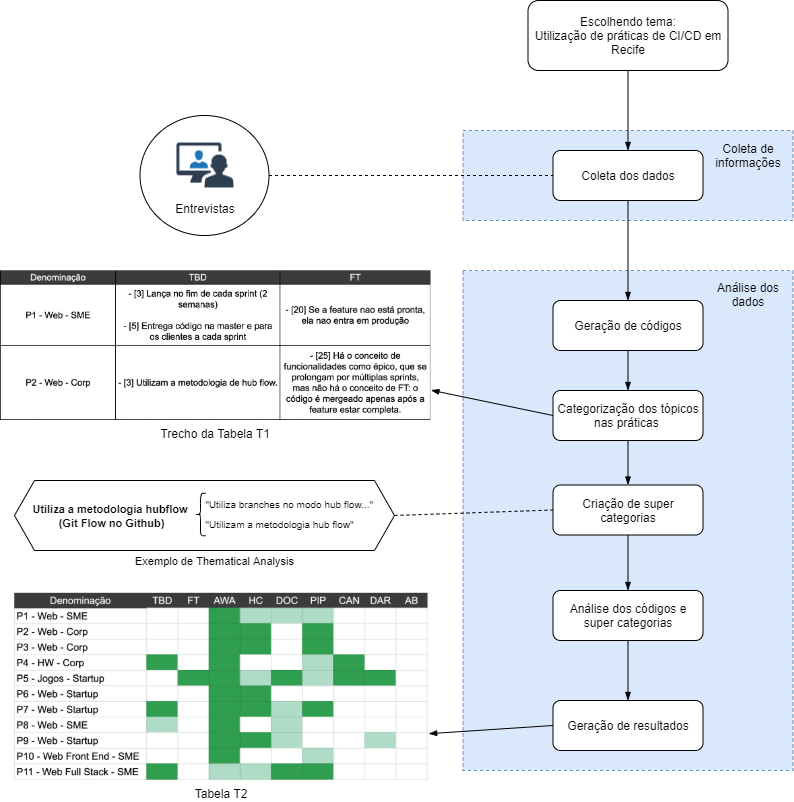
\includegraphics[scale=0.5]{metodologia_tcc.png}
\end{center}
\caption[Fluxograma da Metodologia]{
    Demonstra como funcionou o processo de coleta e análise de dados.
}\label{fluxograma_metodologia}
\end{figure}

    
A \figref{fluxograma_metodologia} apresenta uma visão geral de como funcionou o processo de coleta e análise de dados. A análise foi feita apenas pelo autor deste artigo. O processo escolhido foi baseado nas fases de \emph{Coding} e \emph{Thematic Analysis} da metodologia \emph{Grounded Theory} \cite{groundedTheory}. No processo de Coding a ideia é levantar rótulos ou tags relevantes para o texto e, tradicionalmente, é feito baseado na transcrição das entrevistas. No entanto, neste trabalho o autor gerou códigos através da escuta das entrevistas. Então, como um exemplo, a seguinte citação:

\begin{quotation}[]{P5}
"Como somos uma equipe muito pequena, todos os desenvolvedores são meio que DEVOPS. Quando tem que tomar alguma decisão nós entramos em discussão e definimos por nós."
\end{quotation}

Gerou o código: \emph{"Todos os desenvolvedores são devops."} - P5\_15

É importante salientar que os códigos gerados sofreram um certo enviesamento visto que este trabalho é uma replicação de um estudo, então o autor tinha em mente que assuntos estavam sendo procuradas na fala durante o levantamento de códigos. 

Então, após levantados todos os códigos de uma entrevista, estes foram revisados para garantir semântica e sintaxe adequadas. Alguns códigos nessa fase foram eliminados por redundância, enquanto outros foram quebrados em múltiplos. Depois, eles foram agrupados, quando compatíveis, em cada uma das 9 práticas descritas pelo artigo base e foi escolhida uma nota entre 0 a 2, representando não utiliza, utiliza parcialmente e utiliza completamente baseado nas definições do artigo base traduzidas. Este processo foi então replicado para cada uma das 11 entrevistas.

Ao final do processo ainda haviam 3 ligações entre a prática de \emph{Dark Launch} e entrevistados que não tinham recebido nenhum código em comum. Para estes casos, foi enviado um email diretamente para cada um dos entrevistados com a definição do artigo base da técnica e foi perguntado se o entrevistado utilizava ou não a mesma, o que gerou mais 3 códigos. Ao final, 292 códigos surgiram ao todo.

O agrupamento entre códigos e práticas gerou a Tabela T1, que mostra uma visão geral de cada relação entre prática e entrevistado, contendo a nota dada e os códigos que justificam a nota. Esta tabela contém 147 códigos.

De posse da tabela T1 foi gerada a Tabela T2, que contem uma visão reduzida da primeira, contendo apenas as notas de cada uma das práticas para cada um dos entrevistados com as colunas ordenadas de acordo com o \emph{Stairway to Heaven} descrito no artigo base. Com a Tabela T2, também foi criada uma nova Tabela T3 com o mesmo formato da primeira, mas com as colunas ordenadas pela utilização de cada prática em ordem decrescente. Esta tem como objetivo replicar a Tabela 1 do artigo base \cite{empiricalStudy2016}.

Por fim, para identificar padrões e abstrações nos códigos agrupados na Tabela T1, foi feito um trabalho de agrupamento semântico, gerando por fim a tabela T4 apresentando as novas super categorias geradas no processo de \emph{Thematic Analysis}. Neste, 17 super categorias foram geradas.

É importante salientar que ainda durante o processo de levantamento de códigos surgiram tópicos relevantes que não se relacionavam diretamente com as práticas descritas, mas que são perguntados pelo questionário e relevantes para o tema tratado. Surgiram então 2 novas colunas que agregavam códigos sobre as práticas de \emph{Code Review} e de testes automáticos. Para estas foram relacionados 29 códigos, e duas super categorias foram geradas.

\section{Participantes}

No total foram entrevistados 11 desenvolvedores (P1 a P11) de 7 empresas diferentes sediadas em Recife. Destes, 3 eram mulheres. Pode-se ver a distribuição dos participantes entre gênero na \figref{genero}. Dentro desse grupo, 9 trabalhavam com aplicações Web, enquanto 1 trabalhava com sistemas embarcados e o último, com jogos.

\begin{figure}[ht]
\begin{center}
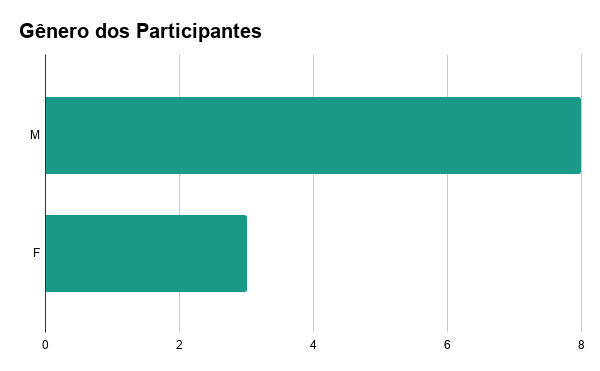
\includegraphics[scale=0.5]{demographics-genero.png}
\end{center}
\caption[Distribuição dos Participantes por gênero]{
    Distribuição dos Participantes por gênero
}\label{genero}
\end{figure}

A escolha dos entrevistados foi feita baseado na rede de conhecidos dos entrevistadores, com o propósito de agregar pessoas de que trabalhavam em empresas de tamanhos distintos para garantir uma variedade de parâmetros envolvidos. Como é possível perceber na \figref{tamanho_empresa}, com relação a esse aspecto a amostra está bem distribuída. 


\begin{figure}[ht]
\begin{center}
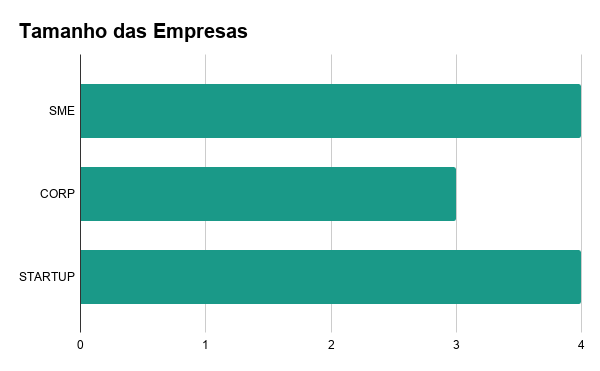
\includegraphics[scale=0.5]{demographics-tamanh-das-empresas.png}
\end{center}
\caption[Distribuição dos Participantes por tamanho da empresa]{
    Distribuição dos Participantes por tamanho da empresa.
}\label{tamanho_empresa}
\end{figure}



\section{Resultados}

Neste capítulo serão apresentados os resultados encontrados com as entrevistas baseadas no processo de análise de dados apresentada no capítulo anterior.

\subsection{Estudo de Predomínio das Práticas}

Com o intuito de responder a pergunta de pesquisa RQ1 -- \emph{Quais as práticas de CI/CD são utilizadas pelas empresas em Recife?} -- de forma restrita aos 11 entrevistados das 7 empresas da amostra, foi montada a Tabela \ref{tabela_t3}, demonstrando a utilização de cada uma das práticas definidas para cada um dos participantes. Nesta, é demonstrada através da coloração da célula o grau de utilização de determinada prática por determinado participante. Assim, o verde mais escuro significa que o participante utiliza totalmente, enquanto o verde claro significa utilização parcial e, por fim, o branco denota a não utilização. Esta foi produzida a partir da Tabela Entrevistado-Pratica-Codigos, retirando-se os códigos agrupados e ordenando as colunas pela utilização de determinada prática. A ideia é replicar a Tabela 1 do artigo base \cite{empiricalStudy2016}, presente na Figura \ref{tabela_1_artigo_base}.

\begin{table}[ht]
\begin{center}
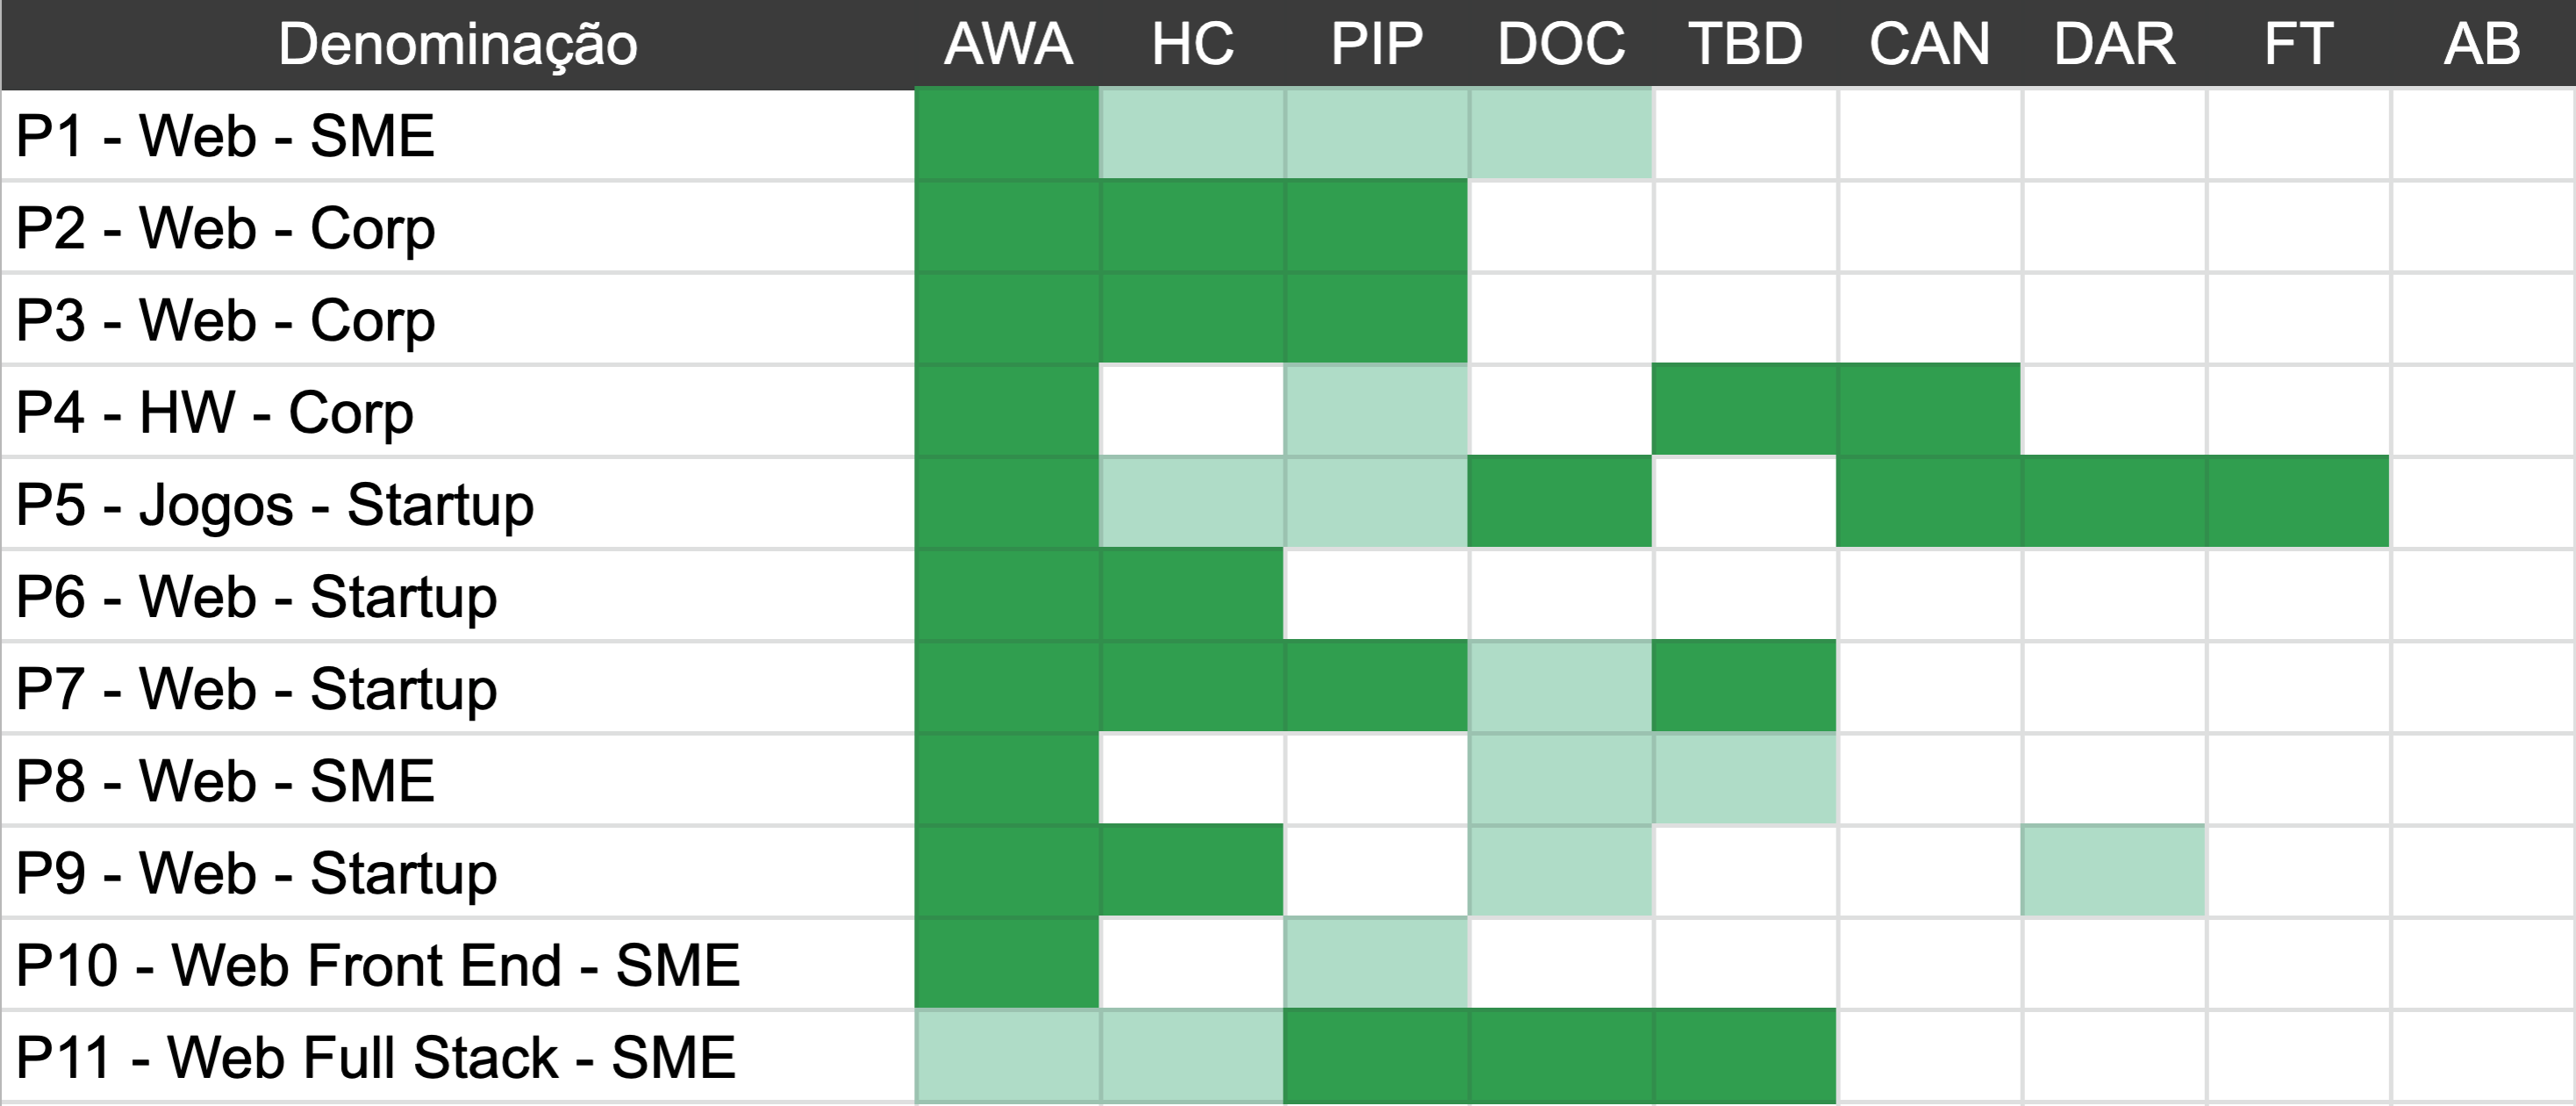
\includegraphics[width=\linewidth]{tabelaT3.png}
\end{center}
\caption[Nível de utilização das práticas, com as colunas em ordem decrescente de uso]{
    Nível de utilização de cada uma das práticas, com as colunas ordenadas em ordem decrescente de uso.
}\label{tabela_t3}
\end{table}

\begin{figure}[ht]
\begin{center}
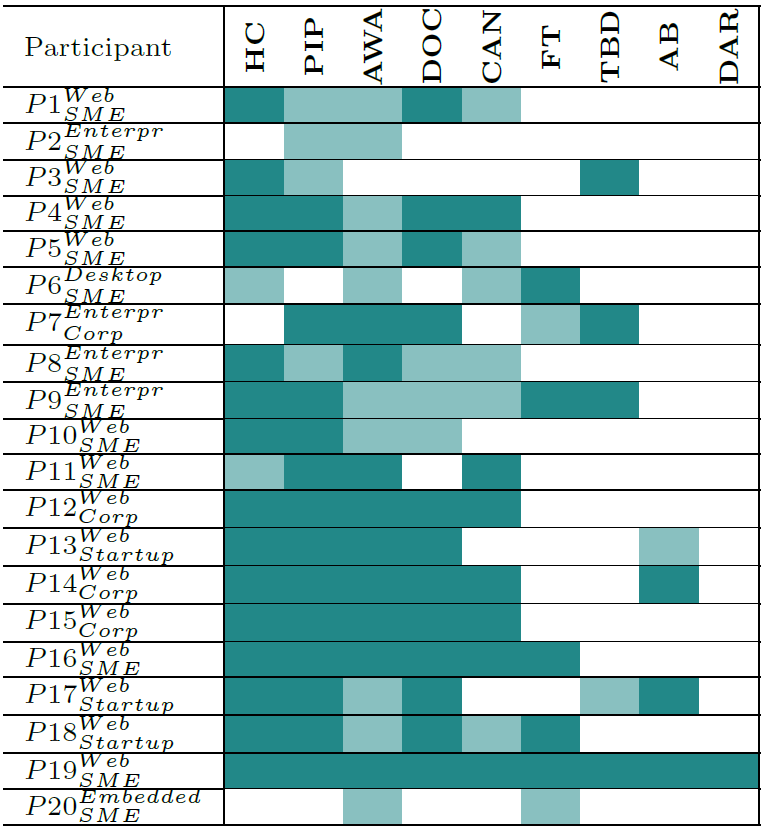
\includegraphics[width=0.9\linewidth]{tabela1-artigo-base.png}
\end{center}
\caption[Tabela 1 do artigo base]{
    Utilização das práticas pelos participantes do artigo base.
    Fonte: Schermman et al \cite{empiricalStudy2016}.
}\label{tabela_1_artigo_base}
\end{figure}

Com a Tabela \ref{tabela_t3} é possível perceber que \emph{Developer awareness [AWA]} foi a prática mais encontrada em toda a amostra, sendo totalmente utilizada pela grande maioria dos entrevistados; apenas um deles utiliza parcialmente. Logo após, pode-se encontrar as práticas de \emph{Health Check} [HC] e Pipeline de Implantação [PIP]  na segunda e na terceira colocação, respectivamente. No geral, também pode-se inferir que as técnicas de \emph{Partial Rollouts} são ainda muito pouco utilizadas, com as 3 práticas do grupo entre as quatro últimas colocadas. Vale a pena citar que nenhum dos entrevistados utiliza, mesmo que precariamente, a técnica de Testes A/B [AB].

Quando comparamos a Tabela \ref{tabela_t3} com a Tabela 1 do artigo base (Figura \ref{tabela_1_artigo_base}), podemos perceber que há diferenças de posição entre práticas, mas que não há mudanças exorbitantes. Com a ajuda da Figura \ref{diferenca_entre_posicoes_fig}, é possível perceber que há uma diferença de no máximo 2 posições na ordem de predomínio, ao comparar os resultados obtidos neste trabalho com os do artigo base. É possível perceber que as práticas de AWA, TBD, DAR e FT tiveram mudanças de 2 posições, enquanto HC, PIP, CAN e AB tiveram apenas diferença de 1 unidade de posição. Apenas \emph{developer on call} permaneceu no mesmo local dentro das duas amostras. Por fim, é interessante perceber que o conjunto das três primeiras práticas é o mesmo, mas em posições trocadas nos dois estudos.

\begin{table}[ht]
\begin{center}
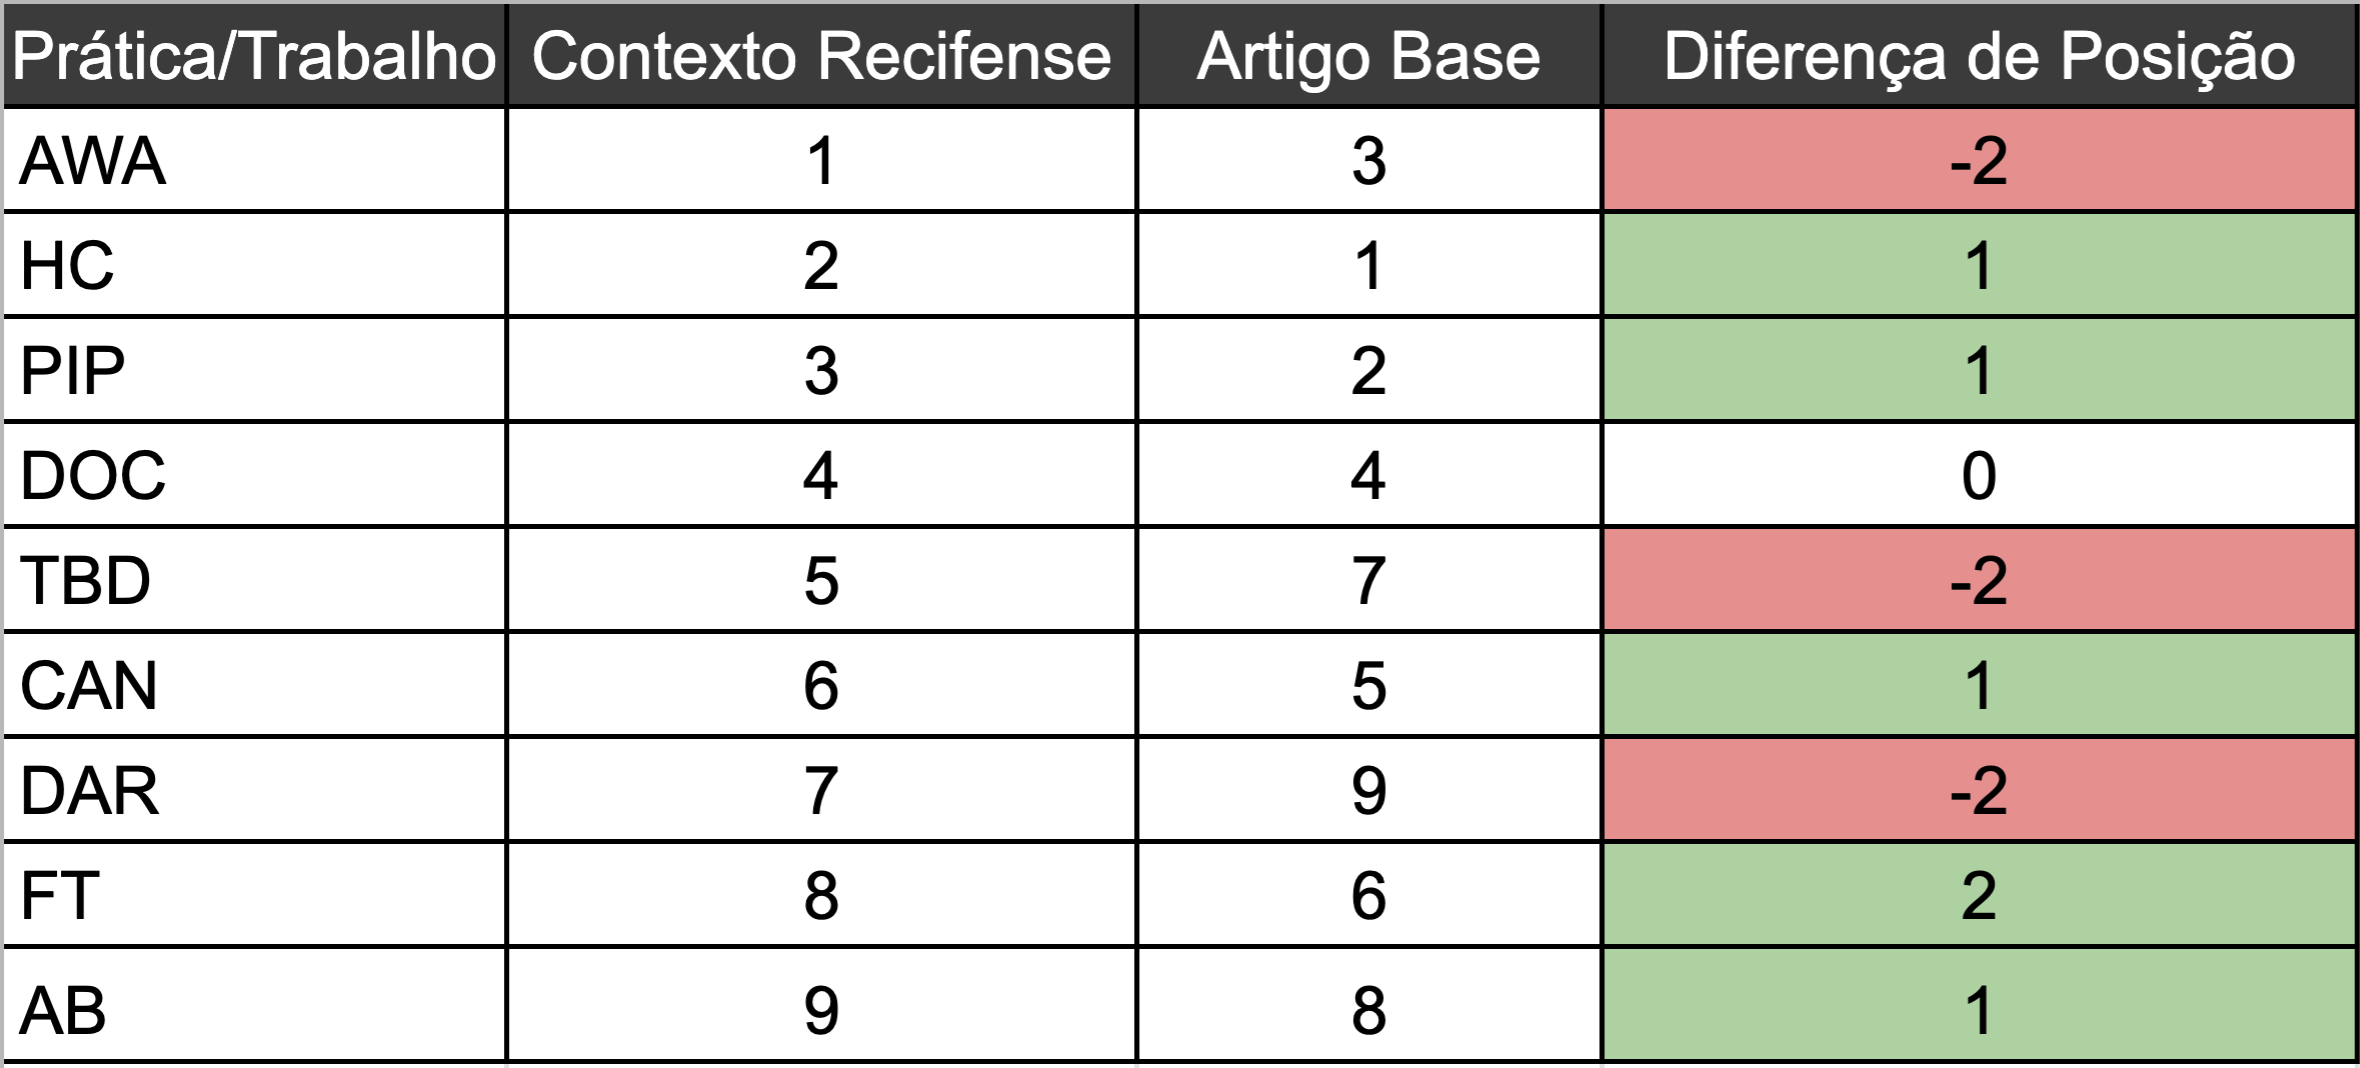
\includegraphics[width=0.9\linewidth]{diferenca_entre_posicoes.png}
\end{center}
\caption[Diferença entre a ordem de predomínio das práticas]{
    Diferença entre o artigo base e este trabalho a respeito da ordem de predomínio das práticas.
}\label{diferenca_entre_posicoes_fig}
\end{table}

\subsection{Stairway to heaven}

Com o objetivo de responder a pergunta de pesquisa RQ2 -- \emph{O cenário de CI/CD nas empresas em Recife segue o ``stairway to heaven'' proposto no artigo?} -- foi produzida a Tabela \ref{tabela_t2}. Esta contém a visualização de utilização das práticas, utilizando a mesma técnica de cores aplicada na Tabela \ref{tabela_t3} e explicada na seção anterior, mas com as colunas ordenadas pela escada definida pela sequência de práticas do \emph{Stairway to Heaven} apresentada na Figura \ref{stairway} (Capítulo 3).

\begin{table}[ht]
\begin{center}
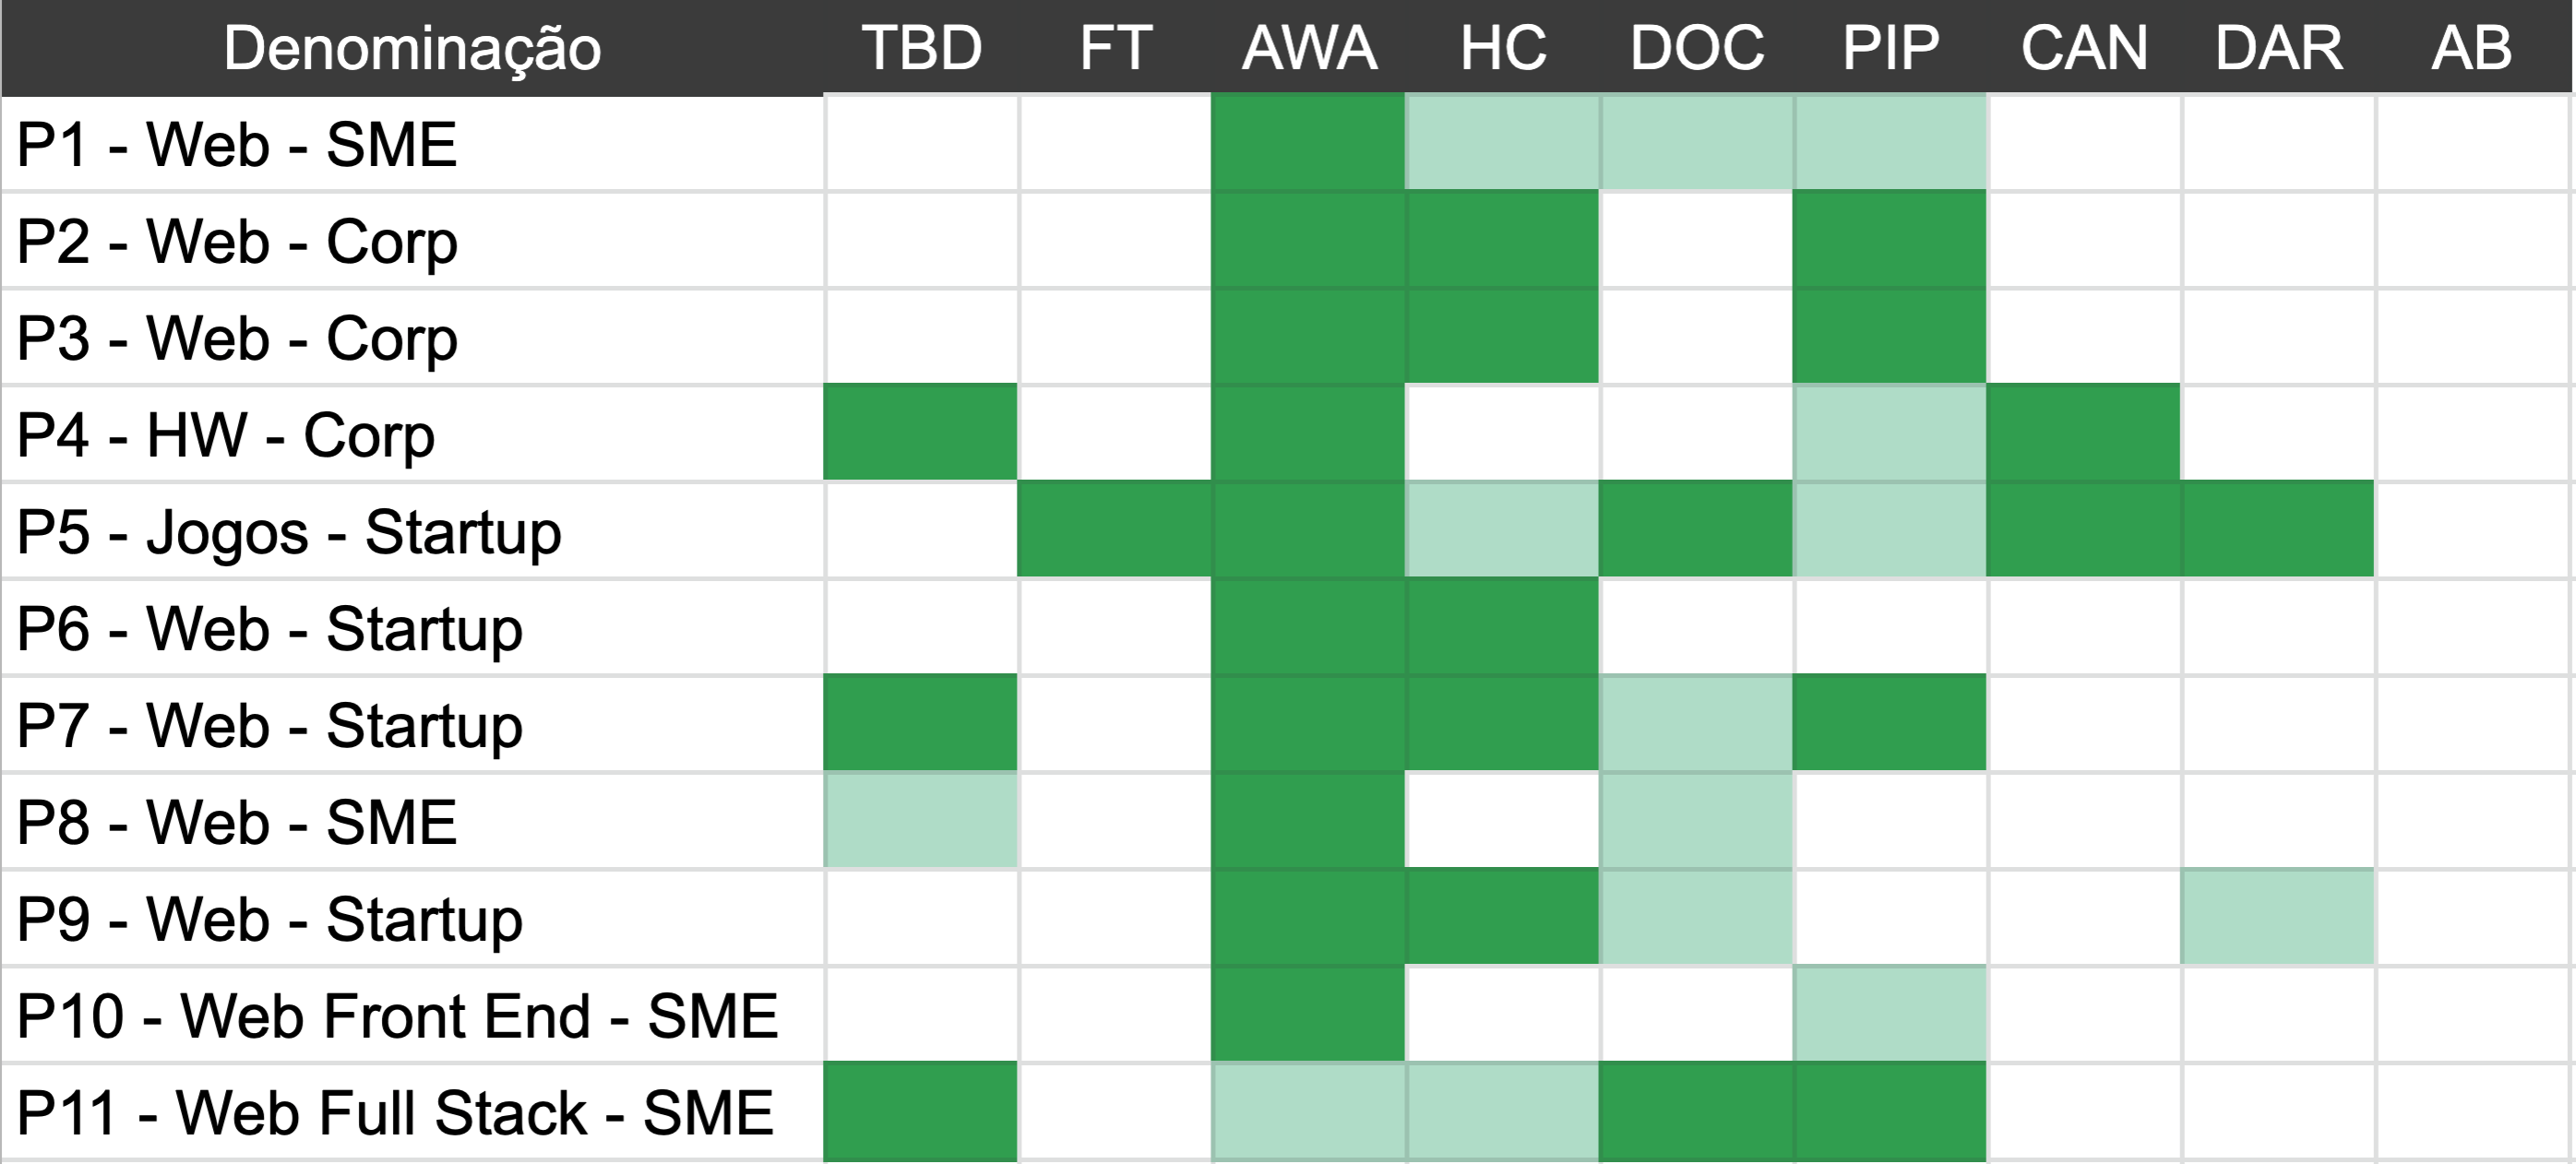
\includegraphics[width=0.95\linewidth]{tabelaT2.png}
\end{center}
\caption[Nível de utilização das práticas, com as colunas na ordem do \emph{Stairway to Heaven}]{
    Nível de utilização de cada uma das práticas, com as colunas ordenadas na ordem do \emph{Stairway to Heaven}.
}\label{tabela_t2}
\end{table}

Com a Tabela \ref{tabela_t2} é possível perceber que a amostra deste estudo, assim como a amostra do estudo original, não segue a evolução proposta pelos autores do artigo base. Isso fica claro quando percebe-se que não há, em nenhum dos entrevistados, uma relação clara entre a coloração da coluna com a sua anterior. É possível notar também que há uma lacuna nas duas primeiras práticas, seguido de uma grande utilização da terceira, confirmando a tese de que a \emph{Stairway to Heaven} não foi identificada na amostra. O mais próximo dos participantes é P5, mas ainda há nele a falta do pilar TBD do primeiro degrau da escada. É interessante destacar que na amostra do próprio artigo base também não foi possível identificar a escada de evolução, como é possível visualizar na Figura \ref{tabela_1_artigo_base}.

\subsection{Análise das Práticas}

Nesta seção será abordado, para cada uma das práticas, as principais curiosidades encontradas na amostra. Esta tem como objetivo responder a pergunta RQ3: \emph{Quais são os princípios e práticas subjacentes que governam a adoção de CI/CD na indústria?}.

Para poder definir padrões encontrados na amostra, o autor, após a fase de agrupamento semântico, juntou todos os códigos e super categorias ligadas a cada uma das práticas, baseando-se principalmente na nota de utilização. Com a leitura e reflexão deste conjunto, o autor procurou por princípios que governam a adoção ou não de cada prática. Foi feito também um estudo comparativo com os resultados obtidos pelo artigo base para analisar discrepâncias e congruências entre os dois contextos de estudo.

\subsubsection{Integração Contínua}

Com a Tabela \ref{tabela_t3} é possível perceber que, apesar da grande disseminação a respeito de informações relacionadas a infraestrutura e manutenção de software -- ligadas à prática de \emph{Developer Awareness} \cite{awa} -- estar em primeiro lugar, as outras técnicas que compõem o conjunto de integração contínua ainda não estão disseminadas na nossa amostra.

\paragraph{Trunk Based Development [TBD]}
Na amostra é possível perceber que a técnica de \emph{Trunk Based Development} [TBD] \cite{devAndDeploymentFB} não é tão amplamente adotada, visto que apenas 4 entrevistados utilizam ao menos parcialmente. Destes, 2 comentam que entregam novas versões aos clientes baseados em novas funcionalidades, e não em \emph{sprints}. Já entre os que não utilizam, 5 integram o código apenas no final da \emph{sprint}. Deste grupo, 2 utilizam a metodologia \emph{Git Flow} \cite{gitFlow}, que define uma maneira de manusear várias branches ao mesmo tempo de modo que os desenvolvedores deparem-se com o mínimo de conflitos possível e que software seja entregue em versões bem definidas.

\paragraph{Feature Toggles [FT]}

No estudo foi possível perceber que, na amostra, a prática de \emph{Feature Toggles} [FT] \cite{featureToggles} é raramente utilizada, assim como no artigo base. Esta técnica foi encontrada apenas na equipe do participante P5, que a utilizava para esconder funcionalidades enquanto testes manuais ainda estavam sendo feitos. Geralmente esta técnica é utilizada para auxiliar a integração de códigos ainda não finalizados quando a equipe utiliza técnicas como o \emph{trunk based development}, mas este não é o caso de P5. É interessante notar que este participante também foi um dos poucos que utilizava a técnica de \emph{Canary Releases} [CAN].

Entre o grupo dos que não utilizavam, 7 só enviam código novo para produção quando a funcionalidade está concluída. Deste grupo, 2 comentaram que fazem uso de conceito de épicos, onde uma história de usuário se prolonga por mais do que apenas uma sprint. É também interessante notar que P3 está em vias de utilizar esta técnica para reduzir conflitos de \emph{merge} e \emph{rebase} devido ao grande número de desenvolvedores em seu time, como podemos ver na citação:


\begin{quote}
    ``O meu time tem 23 [pessoas]. [...] a gente tá trabalhando em funcionalidades muito distintas, então às vezes acontece de termos um paralelismo de branches muito grande. [...] é muito complicado `mergear' e fazer \emph{rebase} de tudo. Realmente dá muitos conflito'' --- P3 -- Web -- CORP
\end{quote}


\paragraph{Developer Awareness [AWA]}

Na amostra é possível identificar que a prática de \emph{Developer Awareness} [AWA] é amplamente adotada nas companhias, assim como na amostra do artigo base. Em 6 entrevistas foi possível perceber que o time de desenvolvimento era o mesmo responsável pela entrega e manutenção da aplicação. Em outras 2, há um time específico de \emph{DevOps}, mas não havia grandes silos entre este e a equipe de desenvolvimento. Um caso interessante foi o de P11, que, apesar de um conhecimento espalhado dentro da equipe, há receio e insegurança por parte de alguns a respeito de questões de infraestrutura no geral.


\subsubsection{Implantação Contínua}

É possível inferir, baseado principalmente na Tabela \ref{tabela_t3}, que as técnicas ligadas ao processo de implantação contínua estão presentes na maioria das equipes da amostra: as 3 estão nas quatro primeiras colocações. 

\paragraph{Health Checks [HC]}

Sobre a prática de \emph{Health Checks} [HC] \cite{devopsBook}, é possível perceber que, apesar de não ser o mais adotado -- como foi no artigo base, ainda tem destaque entre as outras, presente na segunda colocação. Na amostra, 7 entrevistados continham pelo menos uma forma rudimentar de verificação e alertas, e destes, 2 continham apenas verificações não muito complexas. Um ponto interessante que surgiu foi o fato de P4 achar que não era necessário utilizar esta técnica por estar em fase de prototipação.

\paragraph{Developer on Call [DOC]}

Na amostra é possível perceber que a técnica de \emph{Developer on Call} [DOC] \cite{devAndDeploymentFB} é mais adotada de forma implícita do que de fato definida -- 3 entrevistados estão em times que funcionam desta forma. Contudo, 5 pessoas do grupo não utilizam esta prática: alguns comentaram que a confiança nos testes automáticos faz com que não utilizem a prática, enquanto outro comentou que a prática é inclusive mal vista pela empresa.

Uma dicotomia interessante foi encontrada entre os resultados da amostra deste trabalho e o do artigo base. Este último comenta que a prática já está sendo largamente aceita nas organizações atualmente, e inclusive um dos entrevistados comenta que essa responsabilidade de ficar até mais tarde para resolver problemas leva os desenvolvedores a escreverem e testarem seus códigos mais veementemente. Tal argumentação tem como base a seguinte citação retirada do artigo e traduzida:

\begin{quote}
    ``Se você não tem testes suficientes e faz deploy de um código ruim isso vai se voltar contra você pois você estará de plantão e terá que dar suporte a isto.'' --- P14 (do artigo base) -- Web -- CORP
\end{quote}


Contudo, com a seguinte citação de P2, é possível perceber que há um sentimento contrário: confia-se no processo de qualidade e, por isso, não necessitam de plantão.


\begin{quote}
    ``Temos o ciclo de QA, se encontrar alguma coisa a gente vê […] não precisa isso de plantão não.'' --- P2 -- Web -- CORP
\end{quote}

\paragraph{Pipeline de Implantação [PIP]}

Em relação à prática de Pipeline de Implantação [PIP] \cite{devopsBook} é possível inferir que ela é amplamente adotada pela amostra, visto que apenas 2 entrevistados obtiveram nota 0 (não utiliza). No artigo base é possível perceber um resultado semelhante a este. Uma grande parte dos entrevistados segue o mesmo padrão para qualquer tamanho da mudança. Outros 2 tinham alguns processos automatizados, mas a \emph{pipeline} era diferente dependendo do tamanho da mudança.

É interessante perceber que alguns times ainda demonstram falta de automação dos processos da \emph{pipeline}. Isto acontece em decorrência da complexidade da automação, devido às tecnologias e ferramentas utilizadas, ou da falta de prioridade do time para tal.
 
\subsubsection{Entregas Parciais}

Na amostra foi possível perceber que todas as técnicas relacionadas a Entregas Parciais são muito pouco utilizadas: todas estão entre as 4 últimas colocações.

\paragraph{Canary Releases [CAN]}

A técnica de \emph{Canary Releases} [CAN] \cite{continuousDeliveryBook} apareceu nos contextos de jogos e no de sistemas embarcados. Na equipe do entrevistado P5, que trabalha no domínio de jogos eletrônicos, os principais jogadores -- conhecidos como ``baleias'' -- são escolhidos para participar de um \emph{early access} de novas funcionalidades.  Esses testes levam em torno de 1 semana. 

Já na equipe de P4, que trabalha com sistemas embarcados, a prática era necessária devido ao contexto de atuação e às tecnologias utilizadas. Como o sistema que está em fase de prototipação servirá para o contexto médico, vários testes de campo deveriam ser feitos para garantir que todas as funcionalidades estivessem de acordo com o esperado. Para os testes, o cliente que contratou a empresa de P4 escolhia a quantidade de pessoas e local que serviria como validação de funcionalidades.

Entre os entrevistados que não utilizam a prática de \emph{Canary Releases}, 3 têm um ambiente de homologação para testes e validação de requisitos, mas este utiliza dados diferentes dos de produção. Outros 3 comentam que as features são sempre entregues para todos os usuários ao mesmo tempo.


\paragraph{Dark Launches [DAR]}

Do grupo das práticas associadas a Entregas Parciais, \emph{Dark Launches} [DAR] \cite{devAndDeploymentFB} foi a segunda mais utilizada, mas a menos conhecida entre os entrevistados. Isto se confirma com o fato de que 6 entrevistados disseram nunca ter utilizado, e 3 destes disseram especificamente que não conheciam a técnica. Importante notar que no estudo base \cite{empiricalStudy2016} esta é a menos utilizada do grupo de práticas.

\emph{Dark Launches} foi utilizado totalmente por P5 no contexto de jogos para testes manuais, e apenas parcialmente no contexto de WEB por P9 para validações de alguns cenários que dependiam de dados de produção.


\begin{quote}
    ``A gente implementa a funcionalidade mas condiciona a não aparecer para o usuário até que a gente queira.'' --- P5 -- Jogos -- Startup
\end{quote}

\paragraph{Testes A/B [AB]}

A prática de Testes A/B [AB] \cite{testsAB} não foi identificada em nenhum dos participantes. Entre as principais causas levantadas para tal, 4 entrevistados comentaram que não utilizam pela baixa quantidade de usuários ativos no sistema. Outros 2 comentaram que a técnica não se aplicava ao contexto da aplicação. É interessante notar que esses dois motivos estão presentes no artigo base \cite{empiricalStudy2016}, contudo, ao contrário deste, ninguém na amostra comentou sobre problemas na arquitetura como causa para não utilização.


\begin{quote}
    ``O sistema da gente -- apesar de lidar com uma massa de dados muito grande -- não têm tantos usuários, então não faz muito sentido [utilizar testes A/B]....'' --- P2 -- WEB -- Corp
\end{quote}

Outro motivo importante foi levantado por P8, que comenta que aparentemente não existe na empresa o interesse em investir nessa prática. P3 comenta ainda que o time está mais focado em entregar novas funcionalidades, pois a demanda por parte do cliente é muito grande.

\subsection{Descobertas adicionais}

Esta subseção abordará sobre os dois tópicos marginais que foram levantados durante a análise dos dados obtidos pelas entrevistas: \emph{Code Review} e testes automáticos.

\subsubsection{Code Review}

A prática de \emph{Code Review} \cite{codeReview} é bem vista pela maioria dos entrevistados, considerado uma técnica importante e essencial para o controle de qualidade de código. As razões para o uso são diversas, desde de impor boas práticas -- por P7 -- até o compartilhamento e nivelamento do conhecimento -- por P11.

\begin{quote}
    ``... a partir do momento que o sistema vai crescendo, o próprio desenvolvedor não tem a noção de que aquela sua mudança não é a melhor forma de fazer e que pode quebrar outras partes do sistema...'' --- P2 -- WEB -- Corp
\end{quote}

Ainda na amostra, 3 entrevistados acreditam que a prática funciona principalmente para troca de conhecimento. Sobre isso, a entrevistada P10 comenta que agrega muito valor para ela como novata no time, mas acha que adiciona um tempo desnecessário na entrega de funcionalidades por pessoas mais experientes, visto que -- para ela -- a técnica não faria sentido neste caso.

Outro ponto importante foi a distinção entre dois relatos a respeito do engajamento do time com a prática. Enquanto P3 comenta que a equipe dela é bem aberta ao debate e está engajada com o processo, P7 fala que o processo funciona ``mais ou menos'', dependendo do humor dos revisores.

\subsubsection{Testes Automáticos}

Testes automáticos são, no geral, bem vistos e extremamente recomendados pela maioria dos entrevistados como forma de prevenir erros em tempo de execução. Contudo, o participante P2 comenta que ainda é contrário a depender somente deles como garantia de qualidade.

\begin{quote}
    ``... automação [de testes] não resolve todos os problemas [relacionados a garantia de qualidade], ele vai identificar muita coisa, mas tem várias outras que precisamos do olhar de um testador…'' --- P2 -- WEB -- Corp
\end{quote}

Na amostra, 5 entrevistados acreditam que o aumento da cobertura de testes automáticos pode diminuir a quantidade de bugs em produção. Dentro desse grupo, o participante P9 comenta que isto poderia, no entanto, diminuir a velocidade de entregas do time. P5 adicionou ainda que sente que a \emph{sprint} é muito curta e não consegue tempo dentro destas para adicionar testes automáticos.

\subsection{Ameaças a validade}

Mesmo com a metodologia definida e seguida utilizando métodos conhecidos pela comunidade científica, é necessário levantar possíveis ameaças à validade dos resultados encontrados neste trabalho. Uma ameaça plausível é a quantidade relativamente pequena de entrevistas feitas.

É importante salientar também que os códigos gerados durante o processo de codificação das entrevistas sofreram um certo enviesamento visto que este trabalho é uma replicação de um estudo, então o autor tinha em mente que assuntos estavam sendo procurados na fala durante o levantamento de códigos. 

Outra ameaça que deve ser levada em conta é o processo de \emph{coding} realizado. Ele foi feito baseando-se no áudio das entrevistas, e não nos textos transcritos, como geralmente é feito \cite{groundedTheory}. Isso pode tornar os códigos enviesados ou até mesmo significar a falta de códigos importantes que poderiam ter sido levantados pelo processo original. É válido citar que há algumas vertentes que defendem a codificação através do áudio, por preservar a entonação e a intenção do usuário, mas ainda devem ser feitos trabalhos quantitativos na área para validação e melhor definição do processo \cite{listenCode}. 


\chapter{Conclusão}

Está é a minha conclusão



%%
%% The acknowledgments section is defined using the "acks" environment
%% (and NOT an unnumbered section). This ensures the proper
%% identification of the section in the article metadata, and the
%% consistent spelling of the heading.
% \begin{acks}
% TODO escrever isso melhor
% \end{acks}

%%
%% The next two lines define the bibliography style to be used, and
%% the bibliography file.
\bibliographystyle{ACM-Reference-Format}
\bibliography{biblio}

%%
%% If your work has an appendix, this is the place to put it.
\appendix

\end{document}
\endinput
%%
%% End of file
